\documentclass{beamer}
\usetheme{COURS}
\usepackage{tcolorbox}
\usepackage{textpos}
\usetikzlibrary{arrows,automata}


\def\red{\color{red}}
\def\blue{\color{blue}}
\def\green{\color{green}}

\def\opstyle#1{\ensuremath{\operatorname{#1}}}


\title[Algorithmes combinatoires]%
{\bf Grammaires de descriptions d'objets}
\author{\textbf{\Large Florent Hivert}\\[5mm]
  Mél : \texttt{Florent.Hivert@lri.fr}\\
  Adresse universelle : \texttt{http://www.lri.fr/\~{ }hivert}
}
\date{}

\begin{document}
\newcommand{\Count}{\opstyle{count}}
\newcommand{\List}{\opstyle{list}}
\newcommand{\Iter}{\opstyle{iter}}
\newcommand{\Unrank}{\opstyle{unrank}}
\newcommand{\Rank}{\opstyle{rank}}
\newcommand{\First}{\opstyle{first}}
\newcommand{\Next}{\opstyle{next}}
\newcommand{\Random}{\opstyle{random}}

\newcommand{\Concat}{\opstyle{concat}}
\newcommand{\BS}{\opstyle{BitString}}
\newcommand{\Perm}{\opstyle{Perm}}
\newcommand{\Union}{\opstyle{Union}}
\newcommand{\Prod}{\opstyle{Prod}}

\newcommand{\mA}{\mathcal{A}}
\newcommand{\mB}{\mathcal{B}}
\newcommand{\mC}{\mathcal{C}}
\newcommand{\mD}{\mathcal{D}}
\newcommand{\mE}{\mathcal{E}}
\newcommand{\mI}{\mathcal{I}}
\newcommand{\mZ}{\mathcal{Z}}

\newcommand{\Oh}{O}

%***********************************************************************
\frame{\titlepage}
%***********************************************************************
\begin{frame}{Résumé des épisodes précédents}

  On a vu sur des exemples (mots binaires, permutations) plusieurs technique
  pour résoudre les questions classiques de la génération combinatoire:
  \begin{itemize}
  \item Énumération lexicographique;
    \medskip

  \item Décomposition récursive;
    \medskip

  \item itération vs listage pour gagner en complexité.
  \end{itemize}
  \pause\bigskip\bigskip

  \begin{center}
    \textbf{\Large Solution \textit{ad hoc}
      $\Longrightarrow$ solution générique}
  \end{center}
\end{frame}

\begin{frame}{Objectifs : algorithmes génériques}

  \begin{itemize}
  \item Identifier les \textbf{composants de base:}
    \medskip

    $\Longrightarrow$ Singleton, union, produit cartésien, ensemble et
    multiensemble\dots \pause\bigskip

  \item Comprendre comment \textbf{composer} les briques de base:
    \medskip

    $\Longrightarrow$ grammaire de description, classe combinatoire
    \bigskip

  \item $\Longrightarrow$ \textbf{Algorithmes génériques} !
  \end{itemize}
\end{frame}

\section{Union disjointe}
\begin{frame}{Union disjointe}

  \begin{definition}
    On écrit $C = A \sqcup B$ et on dit que $C$ est l'\textbf{union disjointe}
    de $A$ et $B$ si $C = A \sqcup B$ et $A \cap B = \emptyset$.
  \end{definition}
  \pause\bigskip

  Alors:
  \begin{itemize}
  \item $\Count(C) = \Count(A) + \Count(B)$
  \item On peut prendre: $\List(C) = \Concat(\List(A), \List(B))$
  \end{itemize}
\end{frame}

\begin{frame}[fragile]{Itération sur une union disjointe}

  On fixe l'ordre d'énumération tel que
  $$\List(A\sqcup B) := \Concat(\List(A), \List(B))$$
  \bigskip

  Itération en Python:
\begin{listing}{1}
    def iterunion(A, B):
        for a in A:
            yield a
        for b in B:
            yield b
\end{listing}
\end{frame}

\begin{frame}[fragile]{$\First, \Next$ sur une union disjointe}

  $$\List(A\sqcup B) := \Concat(\List(A), \List(B))$$
\begin{listing}{1}
    def first_union(A, B):
        return A.first()

    def next_union(A, B, x):
        if x in A:
            try:
                return A.next(x)
            except StopIteration:
                return B.first()
        else:
            return B.next(x)
\end{listing}
\end{frame}


\begin{frame}[fragile]{$\Rank$ sur une union disjointe}

  $$\List(A\sqcup B) := \Concat(\List(A), \List(B))$$
\begin{listing}{1}
    def rank_union(A, B, x):
        if x in A:
            return A.rank(x)
        else:
            return A.count() + B.rank(x)

    def unrank_union(A, B, i):
        if i < A.count():
            return A.unrank(i)
        else:
            return B.unrank(i - A.count())
\end{listing}
\end{frame}

\begin{frame}{Le principe de l'idée récursive}

  \begin{verse}\bf\color{blue}\LARGE
    Quand on a un'bonne idée, \\
    on l'appliqu'récursivement: \\
    on obtient le plus souvent\\
    une bien meilleure idée !
  \end{verse}
  \pause\bigskip

  \begin{center}
  \bf\LARGE Unions disjointes récursives
  \end{center}
\end{frame}

\begin{frame}{Les chaînes de $n$-bits ayant $k$-bits à $1$}

  Une chaîne de bit non vide commence soit par un $0$, soit par un $1$:
  $$\BS(n, k) = 0\cdot\BS(n-1, k)\ \sqcup\ 1\cdot\BS(n-1, k-1)$$
  Idem triangle de pascal:
  $$\binom{n}{k} = \binom{n-1}{k} + \binom{n-1}{k-1}$$
  \begin{itemize}
  \item $\BS(n, k).\Count() = \binom{n}{k}$ 
  \end{itemize}
\end{frame}

\begin{frame}[fragile]{$\Rank, \Unrank$ pour les chaînes de $n$-bits ayant
    $k$-bits à $1$}

\small
\begin{listing}{1}
def rank_BSnk(x):
    if not x:        # liste vide
        return 0
    if x[0] == 0:
        return rank_BSnk(x[1:])
    else:
        return binom(len(x)-1, sum(x)-1) + rank_BSnk(x[1:])

def unrank_BSnk(n, k, i):
    if n == 0:
        return []
    bn1k = binom(n-1, k)
    if i < bn1k:
        return [0]+unrank_BSnk(n-1, k, i)
    else:
        return [1]+unrank_BSnk(n-1, k-1, i-bn1k)
\end{listing}
\end{frame}


\begin{frame}{Le problème du calcul de la cardinalité}

  \begin{PROBLEM}
    Le calcul récursif des coefficients binomiaux $\binom{n}{k}$ n'est pas
    efficace car on recalcule plusieurs fois la même chose.
    \medskip

    Plus généralement, le calcul récursif des cardinalités sera très
    inefficace pour la même raison.
  \end{PROBLEM}
\end{frame}


\begin{frame}{Parenthèse: mémoization et programmation dynamique}

  \begin{NOTE}
    \begin{itemize}
    \item\textbf{Mémoisation:} on mémorise tous les calculs pendant la
      récursion au momment où on les fait \pause\bigskip

    \item\textbf{Programmation Dynamique:} résoud les sous-problèmes, des plus
      petits aux plus grands en stockant les résultats intermédiaires.
    \end{itemize}
  \end{NOTE}
  \pause\bigskip

  En général, la programmation dynamique est plus efficace mais plus longue à
  mettre en oeuvre: il faut avoir planifié l'utilisation de la mémoire.
\end{frame}

\begin{frame}{Autre exemple: les permutations}

  Les permutés d'un ensemble $X := \{x_1, x_2, \dots, x_n\}$:
  $$\Perm\{1,2,3\} = 
  1\cdot\Perm\{2,3\}\ \sqcup\ 
  2\cdot\Perm\{1,3\}\ \sqcup\ 
  3\cdot\Perm\{1,2\}
  $$
  Plus généralement:
  \begin{NOTE}
    Énumération lexicographique des permutations:
    $$
    \Perm(X) = \bigsqcup_{i=1}^{n} x_i\cdot\Perm(X/\{x_i\})
    $$
  \end{NOTE}
  \begin{itemize}
  \item $\Perm(X).\Count() = |X|!$
  \end{itemize}
\end{frame}

\begin{frame}{Généralisation: permuté d'un multiensemble}

  $$\Perm\{1,1,2,3\} =
  1\cdot\Perm\{1,2,3\}\ \sqcup\
  2\cdot\Perm\{1,1,3\}\ \sqcup\
  3\cdot\Perm\{1,1,2\}
  $$
  \bigskip

  Notation: $\{1,1,2,3\} = 1^22^13^1$
  $$\Perm(1^22^33^1) =
  1\cdot\Perm(1^12^33^1)\ \sqcup\
  2\cdot\Perm(1^22^23^1)\ \sqcup\
  3\cdot\Perm(1^22^3)
  $$

  \begin{NOTE}
    Énumération lexicographique des multi-permutations:
    $$
    \Perm(X) = \bigsqcup_{i=1}^{n} x_i\cdot\Perm(X/\{x_i\})
    $$
  \end{NOTE}
\end{frame}

\begin{frame}{Coefficient multinomiaux:}

  L'union disjointe précédente nous donne l'égalité de cardinaux:
  \begin{multline*}
    \binom{|I|}{i_1,i_2,\dots,i_k} = \binom{|I|-1}{i_1-1,i_2,\dots,i_k} +
    \binom{|I|-1}{i_1,i_2-1,\dots,i_k} + \\ \dots +
    \binom{|I|-1}{i_1,i_2,\dots,i_k-1}
  \end{multline*}
  \pause\smallskip
  On montre alors:
  \[
  \Perm(x_1^{i_1}\dots x_k^{i_k}).\Count() = 
  \frac{(i_1+i_2+\dots+i_k)!}{i_1!i_2!\dots i_k!} =
  \binom{|I|}{i_1,i_2,\dots,i_k}
  \]
\end{frame}

\begin{frame}{Autre application: transmission en codage NRZ}

  Non Return to Zero, Manière très élémentaire pour transmettre de
  l'information sur un ligne:\qquad 0 : -V,\qquad 1: +V

  \[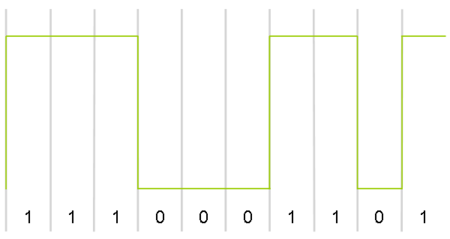
\includegraphics[width=8cm]{media/450px-Nrz.png}\]
  {\small Source: \url{https://fr.wikipedia.org/wiki/Non_Return_to_Zero}}
\end{frame}

\begin{frame}{Perte de synchronisation en codage NRZ}

  Si on envoie une suite trop longue de bits identiques, le récepteur ne
  voit un signal constant. Il ne peut plus se baser sur les transitions pour
  se synchroniser et risque de perdre la synchronisation avec l'émetteur.
  \medskip

  \begin{definition}
    Une séquence de longueur $n$ est dite {\red non-repétitive d'ordre $k$}
    (abréviation $NR_k(n)$) si elle ne contient pas se séquence de plus de
    $k$ bits identiques consécutifs.
  \end{definition}
  On note $NR_k(n, c, i)$ les suites qui commencent par au plus $c$ $i$:
  \begin{itemize}
  \item $NR_k(n, 0, 0) = 1 \cdot NR_k(n-1, k-1, 1)$
  \item $NR_k(n, c, 0) = 0 \cdot NR_k(n-1, c-1, 0)\ \sqcup\ 
               1 \cdot NR_k(n-1, k-1, 1)$
             \item Idem en échangeant les rôles de $0$ et $1$.
  \end{itemize}
\end{frame}


\begin{frame}{C'est un automate fini !}

  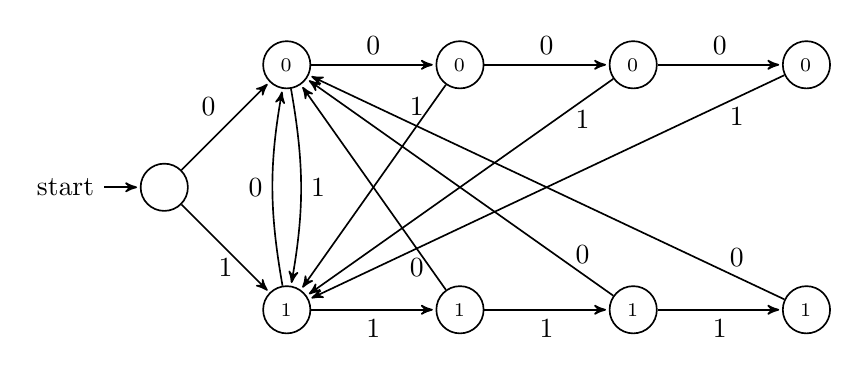
\begin{tikzpicture}[->,>=stealth',shorten >=1pt,auto,node distance=2.2cm,
    semithick]
    \tikzstyle{every state}=[inner sep=1pt, minimum size=6mm]

    \node[initial,state] (I) {$\mI$};
    \node[state] (A0) [above right of=I] {$\mA_0$};
    \node[state] (B0) [right of=A0]      {$\mB_0$};
    \node[state] (C0) [right of=B0]      {$\mC_0$};
    \node[state] (D0) [right of=C0]      {$\mD_0$};
    \node[state] (A1) [below right of=I] {$\mA_1$};
    \node[state] (B1) [right of=A1]      {$\mB_1$};
    \node[state] (C1) [right of=B1]      {$\mC_1$};
    \node[state] (D1) [right of=C1]      {$\mD_1$};
    \path (I)  edge node {0} (A0)
               edge node [below] {1} (A1)
          (A0) edge node {0} (B0)
               edge [bend left=10] node {1} (A1) 
          (B0) edge node {0} (C0)
               edge node [pos=0.2,above] {1} (A1)
          (C0) edge node {0} (D0)
               edge node [pos=0.1,below] {1} (A1)
          (D0) edge node [pos=0.1,below] {1} (A1)
          (A1) edge [bend left=10] node {0} (A0) 
               edge node [below] {1} (B1) 
          (B1) edge node [pos=0.2,below] {0} (A0)
               edge node [below] {1} (C1)
          (C1) edge node [pos=0.1,above] {0} (A0)
               edge node [below] {1} (D1)
          (D1) edge node [pos=0.1,above] {0} (A0) ;
  \end{tikzpicture}
  Tous les états sont acceptants.
\end{frame}

\begin{frame}{Union récursive et automates finis}

  \begin{NOTE}
    La méthode précédente fonctionne pour touts les {\red automates finis
    déterministes}. Soit $\operatorname{Lang}_n(E)$ l'ensemble des mots
    de longueur $n$ acceptés à partir de l'état $E$, alors on a la définition
    récursive:
    \begin{itemize}
    \item Cas de base, pour un état $E$:
      \[
      \operatorname{Lang}_0(E) =
      \begin{cases}
        \{\varepsilon\} & \text{si $E$ est terminal} \\
        \emptyset & \text{sinon}
      \end{cases}
      \]
    \item Étape de la récursion:
      \[
      \operatorname{Lang}_n(E) = \bigsqcup_{E\rightarrow_a E'} a\cdot
      \operatorname{Lang}_{n-1}(E')
      \]
    \end{itemize}
  \end{NOTE}
\end{frame}

\section{Le produit cartesien}
\begin{frame}{Le produit cartésien}

  \begin{definition}
    On appelle \textbf{produit cartesien} de $A$ et $B$ l'ensemble $C$ noté 
    $C:=A\times B$ défini par
    $$C := \{(a,b)\ \mid\ a\in A, b\in B)\}\,.$$
  \end{definition}
  \pause\bigskip

  Alors:
  \begin{itemize}
  \item $\Count(C) = \Count(A)\cdot\Count(B)$
  \item On peut prendre la liste dans l'ordre lexicographique:
    \begin{align*}
      \List(C) = [&(a_0, b_0), (a_0, b_1), (a_0, b_2),\dots, (a_0, b_l),\\
                  &(a_1, b_0), (a_1, b_1), (a_1, b_2),\dots, (a_1, b_l),\\
                  &(a_2, b_0), (a_2, b_1), (a_2, b_2),\dots, (a_2, b_l),\\
                  &\hspace{2.7cm}\dots\hspace{2.7cm}].
    \end{align*}
  \end{itemize}
\end{frame}

\begin{frame}[fragile]{Itération sur un produit cartésien}

  Ordre lexicographique:
  \bigskip

  Itération en Python:
\begin{listing}{1}
    def iter_cartprod(A, B):
        for a in A:
            for b in B:
                yield (a, b)
\end{listing}
\end{frame}

\begin{frame}[fragile]{$\First, \Next$ sur un produit cartésien}

  Ordre lexicographique:
  \bigskip
\begin{listing}{1}
    def first_cartprod(A, B):
        return (A.first(), B.first())

    def next_cartprod(A, B, x):
        (a , b) = x      # pattern matching
        try:
           return (a, B.next(b))
        except StopIteration:
           return (A.next(a), B.first())
\end{listing}
\end{frame}


\begin{frame}[fragile]{$\Rank$ sur un produit cartésien}

  Ordre lexicographique:
  \bigskip
\begin{listing}{1}
    def rank_cartprod(A, B, x):
        (a , b) = x      # pattern matching
        A.rank(a)*B.count() + B.rank(b)

    def unrank_cartprod(A, B, i):
        c = B.count()
        return (A.unrank(i // c), B.unrank(i % c))
\end{listing}
\end{frame}


\section{Notion de classe combinatoire}

\begin{frame}{Notion de classe combinatoire}
  \begin{DEFN}[Classe combinatoire]
    On appelle \textbf{classe combinatoire} un ensemble $\mC$ dont les éléments
    $e$ ont une taille (nommée aussi degrée) noté $|e|$ et tels que l'ensemble
    $\mC_n$ des éléments de taille $n$ est fini:
    \[
    \Count(\{e\in \mC\ \mid\ |e| = n\}) < \infty
    \]
  \end{DEFN}
  Exemple:
  \begin{itemize}
  \item Les mots sur un alphabet où la taille est la longueur
  \item Les permutations de $\{1,\dots n\}$ (taille = $n$)
  \item Les arbres binaires où la taille est le nombre de noeuds
  \end{itemize}
\end{frame}

\section{L'union disjointe graduée}
\begin{frame}{L'union disjointe graduée}

  Si $\mC = \mA \sqcup \mB$, les élements de $\mA$ et $\mB$ gardent leur
  taille dans l'union disjointe graduée:

  \[\mC_n := \mA_n \sqcup \mB_n\]

  Alors:
  \begin{itemize}
  \item $\mC.\Count(n) = \mA.\Count(n) + \mB.\Count(n)$
  \item On peut prendre: $\mC.\List(n) = \Concat(\mA.\List(b), \mB.\List(n))$
  \end{itemize}
  \bigskip\pause

  $\Longrightarrow\quad$ On peut réutiliser tout ce que l'on a vu sur les
  unions disjointes.
\end{frame}

\section{Le produit cartesien gradué}
\begin{frame}{Le produit cartesien gradué}

  Idée : les tailles (complexité, coût, nbr d'emplacements mémoires)
  s'ajoutent.
  \bigskip
  \begin{definition}
    La taille de la paire $(a, b)\in \mA\times \mB$ est la somme des tailles:
    \[|(a, b)|_{\mA\times\mB} := |a|_\mA + |b|_\mB\]
  \end{definition}
\end{frame}

\begin{frame}{Le produit cartesien gradué}

  \begin{NOTE}
    Si $\mC = \mA \times \mB$ alors
    \[
    \mC_n\quad=\quad\bigsqcup_{i+j=n}  \mA_i \times \mB_j
    \]
  \end{NOTE}
  \bigskip\pause

  Calcul de la cardinalité:
  \[
  |\mC_n| = \sum_{i+j=n}  |\mA_i| \times |\mB_j| = 
          \sum_{i=0}^{n}  |\mA_i| \times |\mB_{n-i}|
  \]
  On peut alors prendre l'ordre union/lexicographique suivant:
  \[
  \begin{array}{|c|c|c|c|c|c|}
    \hline
    \mA_0\times \mB_n &     \mA_1\times \mB_{n-1} &  \mA_2\times \mB_{n-2} &  
    \quad\dots\quad &
    \mA_{n}\times \mB_{0}
    \\ \hline
  \end{array}
  \]

\end{frame}

\newcommand{\BinTree}{\opstyle{\mathcal{B}in\mathcal{T}ree}}
\newcommand{\Leaf}{\opstyle{Leaf}}
\newcommand{\Node}{\opstyle{Node}}

\begin{frame}{Application les arbres binaires}

  Spécification récursive:
  \[\BinTree\quad=\quad\Leaf\quad \sqcup\quad \Node(\BinTree\times\BinTree)\]
  \pause\bigskip

  Deux manières de compter les tailles:
  \begin{enumerate}
  \item Nombre de feuille:
  \[\BinTree\quad=\quad\Leaf_1\quad \sqcup\quad \BinTree\times\BinTree\]
  \item Nombre de Noeuds:
  \[\BinTree\quad=\quad\Leaf_0\quad \sqcup\quad \Node_1\times\BinTree\times\BinTree\]
  \end{enumerate}
\end{frame}

\begin{frame}[fragile]{Liste de tous les arbres à $n$~N\oe uds}
   \begin{ALGO}
    \begin{itemize}
    \item \textbf{Entrée:} un entier positif ou nul \texttt{n}
    \item \textbf{Sortie:} une liste d'arbres
    \end{itemize}
\begin{verbatim}
    if n == 0:
        yield arbreVide()
    for i in range(n):
        for g in BinTree(i):
            for d in BinTree(n-1-i):
                yield Noeud(g,d)
\end{verbatim}
  \end{ALGO}
\end{frame}

\begin{frame}{Nombre de Catalan}
  \begin{PROP}
    Le nombre d'arbres binaires à $n$ n\oe uds est appelé $n$-ième nombre de
    Catalan noté $C_n$. Les nombre de Catalan vérifient la récurrence:
    \begin{equation*}
      C_0=1\qquad C_n = \sum_{i=0}^{n-1} C_i C_{n-1-i}\,.
    \end{equation*}
    On peut trouver une formule close:
    \begin{equation*}
      C_n = \frac{(2n)!}{n!(n+1)!}\,.
    \end{equation*}
  \end{PROP}
  Voici les premières valeurs:
  \[C_0=1,\ C_1=1,\ C_2=2,\ C_3=5,\ C_4=14,\ C_5=42,\ c_6=132\,.\]
\end{frame}

\section{Specification d'une classe combinatoire}
\begin{frame}{Specification d'une classe combinatoire}

  But: on veut décrire une \textbf{classe combinatoire} de manière à pouvoir
  appliquer automatiquement les algorithmes de comptage, itération,
  génération,\dots.
  \bigskip

  Pour ceci, on va utiliser une \textbf{grammaire} qui code comment appliquer
  récursivement les constructions précédentes.
\end{frame}

\begin{frame}{Specification d'une classe combinatoire}
\begin{NOTE}[Grammaire de description d'objets]
  Constructeurs terminaux:
  \begin{itemize}
  \item $\mE(o)$ : la classe qui contient un seul objet $o$ de taille $0$
  \item $\mZ(o)$ : la classe qui contient un seul objet $o$ de taille $1$
  \end{itemize}
  Constructeurs binaires:
  \begin{itemize}
  \item $\mC = \Union(\mA, \mB)$ : union disjointe graduée:
    \[|a|_\mC = |a|_\mA\ \text{si $a\in\mA$}\qquad
      |a|_\mC = |b|_\mB\ \text{si $b\in\mB$}\]
  \item $\mC = \Prod(\mA, \mB)$ : produit cartésien graduée:
    \[|(a, b)|_\mC = |a|_\mA + |b|_\mB\ \text{si $a\in\mA$ et $b\in\mB$}\]
  \end{itemize}
\end{NOTE}
\end{frame}

\begin{frame}{Exemples:}

  \begin{itemize}
  \item Les arbres binaires, la taille est le nombres de \textbf{Noeuds}
    \[
    \BinTree = \Union(\mE(\bot), \Prod(\mZ(\circ), \Prod(\BinTree, \BinTree))
    \]
  \item Les arbres binaires, la taille est le nombres de \textbf{Feuilles}
    \[
    \BinTree = \Union(\mZ(\bot), \Prod(\BinTree, \BinTree))
    \]
  \end{itemize}
\end{frame}

\begin{frame}{Exemples: Codage d'un automate fini}

\hspace{2.2cm}
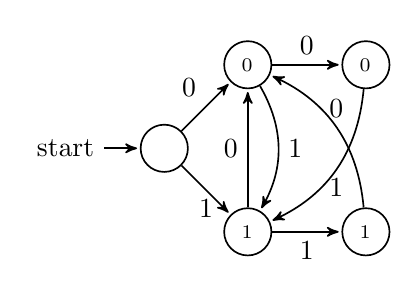
\begin{tikzpicture}[->,>=stealth',shorten >=1pt,auto,node distance=1.5cm,
                    semithick]
  \tikzstyle{every state}=[inner sep=1pt, minimum size=6mm]

  \node[initial,state] (I)                     {$\mI$};
  \node[state]         (A0) [above right of=I] {$\mA_0$};
  \node[state]         (B0) [right of=A0]      {$\mB_0$};
  \node[state]         (A1) [below right of=I] {$\mA_1$};
  \node[state]         (B1) [right of=A1]      {$\mB_1$};
  \path (I) edge node {0} (A0)
            edge node [below] {1} (A1)
        (A0) edge node {0} (B0)
             edge [bend left] node {1} (A1)
        (A1) edge node {0} (A0)
             edge node [below] {1} (B1)
        (B0) edge [bend left] node [below] {1} (A1)
        (B1) edge [bend right] node [above] {0} (A0)
  ;
\end{tikzpicture}

  Les mots binaires qui n'ont pas plus de deux lettres identiques
  consécutives:
  \begin{align*}
    \mI &= \mE(\varepsilon)\ \sqcup\
         (\mZ("0")\times\mA_0)\ \sqcup\ (\mZ("1")\times\mA_1)\\
    \mA_0 &= \mE(\varepsilon)\ \sqcup\
         (\mZ("0")\times\mB_0)\ \sqcup\ (\mZ("1")\times\mA_1)\\
    \mB_0 &= \mE(\varepsilon)\ \sqcup\ (\mZ("1")\times\mA_1)\\
    \mA_1 &= \mE(\varepsilon)\ \sqcup\
         (\mZ("0")\times\mA_0)\ \sqcup\ (\mZ("1")\times\mB_1)\\
    \mB_1 &= \mE(\varepsilon)\ \sqcup\ (\mZ("0")\times\mA_0)\\
  \end{align*}
\end{frame}


\begin{frame}{Exemples: Codage d'un automate fini}

\hspace{2.2cm}
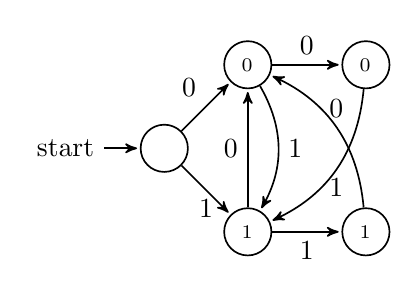
\begin{tikzpicture}[->,>=stealth',shorten >=1pt,auto,node distance=1.5cm,
                    semithick]
  \tikzstyle{every state}=[inner sep=1pt, minimum size=6mm]

  \node[initial,state] (I)                     {$\mI$};
  \node[state]         (A0) [above right of=I] {$\mA_0$};
  \node[state]         (B0) [right of=A0]      {$\mB_0$};
  \node[state]         (A1) [below right of=I] {$\mA_1$};
  \node[state]         (B1) [right of=A1]      {$\mB_1$};
  \path (I) edge node {0} (A0)
            edge node [below] {1} (A1)
        (A0) edge node {0} (B0)
             edge [bend left] node {1} (A1)
        (A1) edge node {0} (A0)
             edge node [below] {1} (B1)
        (B0) edge [bend left] node [below] {1} (A1)
        (B1) edge [bend right] node [above] {0} (A0)
  ;
\end{tikzpicture}

Dans cet exemple: plus simple, on inclut la lettre dans l'état:
  \begin{align*}
    \mI &= \mE(\varepsilon)\ \sqcup\ \mA_0\ \sqcup\ \mA_1\\
    \mA_0 &= \mZ("0") \times (\mE(\varepsilon)\ \sqcup\ \mB_0 \sqcup\ \mA_1)\\
    \mB_0 &= \mZ("0") \times (\mE(\varepsilon)\ \sqcup\ \mA_1)\\
    \mA_1 &= \mZ("1") \times (\mE(\varepsilon)\ \sqcup\ \mB_1 \sqcup\ \mA_0)\\
    \mB_1 &= \mZ("1") \times (\mE(\varepsilon)\ \sqcup\ \mA_0)\\
  \end{align*}
\end{frame}

\end{document}

%%% Local Variables:
%%% mode: latex
%%% TeX-master: t
%%% End:
